\chapter{Test and Evaluation} \label{sec:tests}

When conceptualizing the tests to be performed, in order to evaluate and validate the solution, the main consideration was to understand how well the solution performed with the constrains made in the hardware and software.

From the moment the final design of the smart shelve was decided, it was evident that two problems could compromise the performance of the solution: the metal structure of shelve and the old, not maintained, Fosstrak open-source software.

In this chapter will be presented a few tests designed to hint how this problems can compromise this solution. The tags were attached to empty sleeves, representing an ideal test environment~\footnote{It was not possible to attain sleeves with aluminum capsules for testing. They would certainty interfere with the following test results, but not accounted in the work of this dissertation.}.

% specify better the test reader configurations used

\section{Tag orientation} \label{sec:test1}

Prior to the implementation of the solution, an \ac{rf} analysis of tag orientation in shelve was conducted.
The objective was to evaluate the optimal tag orientation in stored products, and provide notions on system reading performance early in the development.
The tags were tested in tree different orientations, illustrated in figure~\ref{fig:tagorientations}.

\begin{figure}
    \centering
    \caption{Tag orientation tested in this dissertation: horizontal, lateral and vertical, respectively}
    \label{fig:tagorientations}
\end{figure}


This test was only executed on the bottom shelve, since the results could be inferred to the others. The bottom shelve also presented the major challenges and could : it had to operate in the \emph{near-field} and was too close to the antenna, which could cause miss readings in the outer laterals due to the beam width.

The test was conducted by dividing the bottom shelve into $18$ quadrants and measure \ac{rssi} values, referent to a single tag, within those quadrants, with a transmission power of $30$dBm and maximum sensitivity of $-80$dBm. The \ac{rssi} results are a mean value calculated from $1000$ values sampled from each quadrant in a uniform motion, repeated in same manner between quadrants.

The results are shown in figure~\ref{fig:tagorientationsresults} in heatmap plots.
They do not represent the obstructions spread across the shelve. These obstructions prevent tag readings, which were not accounted in this test. Obstructions will be evaluated in the next test.

From the results obtained, there is no clear superior orientation. The circular Keonn Advantenna-p14 in conjunction with the \ac{rf} signal deformations caused by the metal structure, make a good job in providing orientation independence.

\begin{figure}
    \centering
    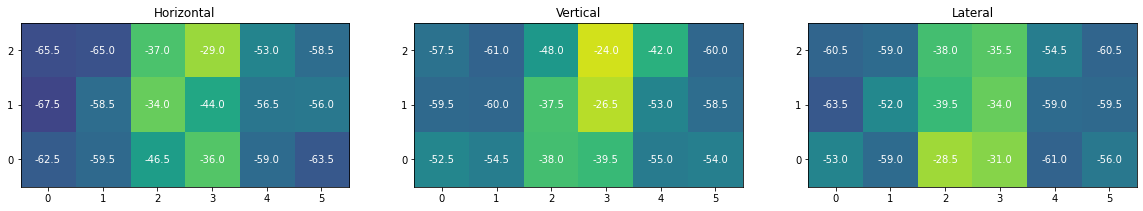
\includegraphics[width=\textwidth]{figs/tests/RSSI_shelve1.png}
    \caption{Tag \ac{rssi} reading results for the different considered orientation. Greater \ac{rssi} values are better.}
    \label{fig:tagorientationsresults}
\end{figure}

A few peculiar observations from the tests are described next:

\begin{itemize}
    \item Horizontal orientated tags have reading problems near the shelf outside metal structure;
    \item Vertical orientated tags, in contrast with horizontal orientated ones, have good reading values near the shelf outside metal structure. They present problems placed on top of the metal bars used to support the shelves.
    \item Lateral orientated tags present difficulty in reader on top of the support metal bars and really close to conners.
\end{itemize}

No major benefits were presented by any orientation.
Theoretically, the lateral tag orientation would present most problems, being parallel to the axis of propagation.
In order to test the system in the most extreme conditions, the lateral orientation was used for sleeves throughout the dissertation and horizontal orientation for product cases for transport.

\section{Shelve \acs{rf} Survey}

The objective of this test was to study and evaluate the certainty and quality of tag readings, by making an \ac{rf} survey of the shelve, with the lateral tag orientation defined previously.
It aims at evaluating the \ac{rf} obstructions present in the solution, which were not considered in the first test.
The results should offer a good representation of the \ac{rf} environment in the shelve and what it could be expected from tag readings in certain locations. 
From the previous test, in section~\ref{sec:test1}, it was observed that the \ac{rssi} does not change when a single tag is placed in one location, allowing the sampling of a single \ac{rssi} value per location. 

The test consisted, once again, in dividing the shelves into quadrants and measure \ac{rssi} values within those quadrants. This time, each shelve was divided in $140$ quadrants ($20\times7$ grid) to have a better perspective of \ac{rf} obstructions. The transmission power and sensitivity were maintained from the previous test.
The results can be seen in figure~\ref{fig:rfsurvey}.

\begin{figure}
    \centering
    \caption{Heatmap of the \ac{rf} survey measured of each shelf with lateral tag orientation}
    \label{fig:rfsurvey}
\end{figure}

It is possible to observe the obstructions caused from the metal bars used to support the middle of each shelf. The surrounding metal structure does not seem to interfere significantly to the point of blocking readings.

\section{Singulation stress test}

This test aim at complementing the observations from previous test by evaluating how the obstructions affect readings of a group of tags placed on top \ac{rf} ``blind'' zones.

The test method consist of selecting locations were obstructions are prevalent and for each one, at a time, place boxes full of sleeves in those positions to evaluate for miss readings, as shown in figure~\ref{fig:sleevepacking}.

From this test was possible to retrieve some interesting observations. 
As expected, \ac{rf} obstruction cause miss readings, but the phenomenon is not as linear as the previous tests with a single tag. 
Some locations did not present miss readings. In those locations, when a sleeve was removed from the case for transport, a tag would miss read, illustrated in figure~\ref{fig:missreading}. The ``disappearing'' tag could be right next to the removed one or in other box, not being evident the obstruction phenomenon happening.
The phenomenon can be linked to:

\begin{itemize}
    \item \ac{rf} obstructions resulting from the presence of \ac{rf}-opaque or \ac{rf}-absorbent objects which block and absorb \ac{rf} waves respectively~\cite{lahiriRFIDSourcebook2005};
    \item ``Re-radiating'' phenomenon due to the \emph{near-field} Fresnel region reacting with the metal structure and the tags antennas~\cite{ElectromagneticRadiationField};
    \item Tag-to-tag interference.
\end{itemize}

\begin{figure}
    \centering
    \caption{Non linear obstruction phenomenon illustration of miss reading caused by the removal of another}
    \label{fig:missreading}
\end{figure}

More research and tests have to be performed in order to confirm these hypotheses.
To complement the observations in these tests, a few metal objects were placed on the shelve, namely a aluminum notebook computer, an aluminum window frame, and a steel oil heater.
The aluminum notebook and window placed in different locations, would interfere with the tag readings. The steel oil heater placed leaning on the shelve did not seem to interfere in any way, indicating a good, confined to the shelve, \ac{rf} radiation.

\section{Operational test}

For the final test, the objective is to validate the platform.
The test consists of make inventory changes and validate through the web interface and database entries if the data is in accordance with those changes, namely if tags added and removed are adequately identified.

The platform was able to adequately read the inventory changes, publish them to the \ac{epcis} repository and be visualized in the web management interface.

\subsection{Problems}

Some of the problems of the software platform were already hinted throughout this dissertation, namely in section~\ref{sec:softwareplatformoptions}.
The Fosstrak software components used in this dissertation are not maintain and this presented the most problems in this dissertation, many which could not be solved.
Modern Java and Tomcat versions created breaking changes in the code, which forced the use of old versions. 
These old versions also do not seem to solved the problems, but reduce the amount of bugs to a point poorly working. A few major problems will be presented next.

Starting with the \ac{fc} middleware, it presents multiple problems. 
The web-based client is broken. The static logical reader definitions is broken.
The standalone client works, but when registering \acp{lrspec} and \acp{ecspec}, most of the times, causes the server to break due to concurrent modification thread error. 

The capture application also presents problems.
The connection between the \ac{ale} interface of the capture application and the middleware seems to have some problems. Using the middleware log information, it is possible to verify that the middleware processes the reports, delivered by the reader, but they are not received or processed by the capture application.
Further inspection on the capture application can not be done due to inexistent log files in the service.
The Drools engine used by the capture application is also old with complex mechanism. Development of complex business logic was a challenge, even with support of experienced users.

Regarding the \ac{epcis} repository, the subscriptions drop \ac{epcis} data with no apparent reason. The \ac{epcis} database also has some problems with modern versions of the mySQL image.

These were the issues present in the final build of the platform. The most time consuming, by far, in this dissertation, was to fix these type of problems, changing Java and Tomcat versions, docker images, containerization configurations, analyzing log files, configurations, to say a few.